% Provenance (never printed): old premiere S material on the lithosphere and the
% asthenosphere (chemical and mechanical layers, the low-velocity zone, the
% geotherm, isostasy); see sources/book2/PROVENANCE.md. S speeds from
% figdata/grade-11/prem_profiles.py (part upper), the geotherm and the solidus
% from geotherm_solidus.py, the elevations from hypsometry.py (ETOPO1).
% Glacial rebound belongs to g12; lithostatic pressure (term) to g12.
\chapter{الغلاف الصخري والغلاف اللدن}\label{ch:g11:lithosphere-asthenosphere}

تسعة أعشار الجبل الجليدي تحت الماء: فالجليد يطفو لأنه أقل كثافة
بقليل من البحر، وهو يغوص في الماء حتى يصير وزن الماء الذي
يزيحه مساويًا لوزن الجبل الجليدي كله. والسلاسل الجبلية تتصرف
على النحو نفسه تقريبًا. فتحت أعلاها تكون القشرة أسمك من المعتاد
بنحو الضعف، ومعظم هذه القشرة الزائدة مختبئ في الأسفل، كالجليد الذي تحت
خط الماء. لكن الجبل الجليدي يطفو في سائل، والوشاح الذي تحت
السلسلة الجبلية صخر صلب. يبيّن هذا الفصل كيف يمكن لجسم صلب أن يتصرف
كمائع يطفو عليه الغلاف الخارجي للأرض، وما هذا الغلاف.
% ledger: usgs:ice-density, karplus:tibet-moho, cm95:crust

\begin{recall}
للأرض قشرة ووشاح ولب (الكتاب 1، الصف 6). ويقع \omterm{def:g11:seismic-structure:moho}{الموهو}، عند
قاعدة القشرة، على عمق نحو \qty{41}{km} تحت القارات في
المتوسط وعلى بضعة كيلومترات تحت قاع المحيط؛ والسرعات الزلزالية
والكثافات معروفة عند كل عمق من \omterm{def:g11:seismic-structure:reference-model}{نموذج مرجعي للأرض}
(\cref{ch:g11:seismic-structure}). ويسخن الصخر مع العمق، بنحو
25 إلى \qty{30}{\celsius} لكل كيلومتر قرب السطح (الكتاب 1، الصف 6).
والجسم الطافي في سائل يزيح من السائل وزنًا يساوي
وزنه، والضغط عند قاع عمود من مادة هو وزن
العمود مقسومًا على مساحته (كتب الفيزياء).
\end{recall}
% ledger: cm95:crust, usgs:crust-thickness, usgs:gradient-29 (Book 1 rows)

\begin{omfigure}
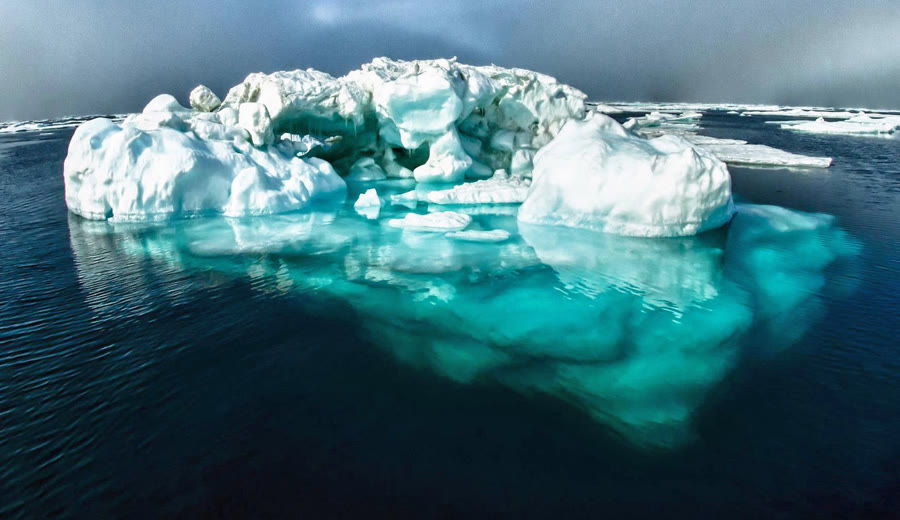
\includegraphics[width=0.66\linewidth]{images/book2/g11-noaa-iceberg.jpg}

{\small جبل جليدي يُرى من فوق الماء مباشرة: الجليد الذي تحت السطح،
والذي يظهر عبر البحر الصافي، أكبر بكثير من الجزء الذي في الهواء.
الصورة: الإدارة الوطنية للمحيطات والغلاف الجوي (ملك عام).}
\end{omfigure}
% ledger: photo:g11-iceberg

\section{طريقتان لتقسيم الأرض إلى طبقات}

القشرة والوشاح واللب طبقات من \emph{مواد}
مختلفة: فالقشرة مصنوعة من صخور غنية بالسيليكون والألومنيوم
والأكسجين، والوشاح من صخر أكثف، واللب من فلز. لكن الجزء الخارجي من
الأرض يمكن تقسيمه أيضًا بحسب \emph{سلوك} صخره حين تؤثر فيه قوى
زمنًا طويلًا جدًا.

\begin{definition}[الغلاف الصخري؛ الغلاف اللدن]\label{def:g11:lithosphere-asthenosphere:lithosphere}
\emph{الغلاف الصخري}\index{غلاف صخري} هو الغلاف الخارجي الصلب
للأرض: القشرة وأعلى جزء من الوشاح وأبرده، وهما معًا
يتكسران إلى الصفائح التكتونية ولا ينسابان. أما
\emph{الغلاف اللدن}\index{غلاف لدن} فهو طبقة الوشاح الواقعة تحت
الغلاف الصخري، وهي أسخن وأضعف، وتنساب
ببطء على امتداد فترات زمنية طويلة، كعجينة شديدة القساوة.
\end{definition}

يقع الحد بين الاثنين على عمق نحو 70 إلى \qty{100}{km} تحت
المحيطات ومعظم القارات، وأعمق تحت أقدم أجزاء
القارات؛ فعبر الولايات المتحدة، مثلًا، يتراوح سمك \omterm{def:g11:lithosphere-asthenosphere:lithosphere}{الغلاف الصخري} بين
نحو \qty{40}{km} في الغرب وأكثر من \qty{200}{km} في
وسط القارة. وقاعدة \omterm{def:g11:lithosphere-asthenosphere:lithosphere}{الغلاف الصخري} ليست \omterm{def:g11:seismic-structure:moho}{الموهو}: فمعظم
\omterm{def:g11:lithosphere-asthenosphere:lithosphere}{الغلاف الصخري} صخر وشاحي.
% ledger: rs09:lab, fischer:lab, porter:lab, usgs:lithosphere-80km (Book 1 row)

\begin{omfigure}
\begin{tikzpicture}[x=1cm, y=-0.0125cm, font=\footnotesize]
% depths to scale: crust 41 km (cm95:crust), lithosphere 100 km (rs09:lab), 0-400 km
  \shade[top color=omLithPeridotite!70, bottom color=omLithPeridotite!25] (5,100) rectangle (8,400);
  \fill[omLithGranite!55] (0,0) rectangle (3,41);
  \fill[omLithPeridotite!55] (0,41) rectangle (3,400);
  \fill[black!25] (5,0) rectangle (8,100);
  \draw (0,0) rectangle (3,400);
  \draw (5,0) -- (5,400) (8,0) -- (8,400) (5,0) -- (8,0);
  \draw[line width=0.8pt] (0,41) -- (3,41);
  \draw[line width=0.8pt, densely dashed] (5,100) -- (8,100);
  \draw[densely dotted, black!60] (3,41) -- (5,41);
  \node at (1.5,20) {القشرة};
  \node[align=center] at (1.5,220) {الوشاح};
  \node[align=center] at (6.5,50) {الغلاف الصخري\\صلب};
  \node[align=center] at (6.5,180) {الغلاف اللدن\\ضعيف، ينساب ببطء};
  \node[align=center, text=black!70] at (6.5,340) {الوشاح الأعمق};
  \node[anchor=south, font=\small] at (1.5,0) {بحسب المادة};
  \node[anchor=south, font=\small] at (6.5,0) {بحسب السلوك};
  \foreach \d in {0,100,200,300,400} {\draw (-0.1,\d) -- (0,\d); \node[anchor=east] at (-0.1,\d) {\d};}
  \node[anchor=east, rotate=90, anchor=south] at (-0.9,200) {\foreignlanguage{arabic}{العمق \babelsublr{(\unit{km})}}};
  \node[anchor=south, font=\scriptsize, align=center] at (4,41) {الموهو\\(\qty{41}{km})};
  \node[anchor=west, align=left] at (8.15,100) {قاعدة\\الغلاف الصخري\\\foreignlanguage{arabic}{على عمق نحو \babelsublr{\qty{100}{km}}}};
\end{tikzpicture}

{\small أعلى \qty{400}{km} من الأرض تحت قارة، بمقياس رسم حقيقي.
في اليسار: الطبقات بحسب المادة. في اليمين: الطبقات بحسب السلوك. ويحوي
\omterm{def:g11:lithosphere-asthenosphere:lithosphere}{الغلاف الصخري} الصلب القشرة كلها وأعلى الوشاح؛ وليس
\omterm{def:g11:lithosphere-asthenosphere:lithosphere}{للغلاف اللدن} حد سفلي حاد.}
\end{omfigure}

\section{نطاق السرعة المنخفضة}

تكشف الموجات الزلزالية \omterm{def:g11:lithosphere-asthenosphere:lithosphere}{الغلاف اللدن}. ففي كل مكان تقريبًا من الأرض تزداد
السرعات الزلزالية مع العمق، لأن الصخر يزداد انضغاطًا. أما تحت
\omterm{def:g11:lithosphere-asthenosphere:lithosphere}{الغلاف الصخري} فيحدث العكس.

\begin{definition}[نطاق السرعة المنخفضة]\label{def:g11:lithosphere-asthenosphere:lvz}
\emph{نطاق السرعة المنخفضة}\index{نطاق السرعة المنخفضة} هو طبقة
الوشاح العلوي، تحت \omterm{def:g11:lithosphere-asthenosphere:lithosphere}{الغلاف الصخري}، التي تنتقل فيها الموجات الزلزالية أبطأ
منها في الصخر الذي فوقها والذي تحتها.
\end{definition}

في \omterm{def:g11:seismic-structure:reference-model}{النموذج المرجعي للأرض}، تنخفض سرعة \omterm{def:g11:seismic-structure:body-waves}{الموجات S} ببطء من \omterm{def:g11:seismic-structure:moho}{الموهو} حتى
\qty{220}{km}، ثم تقفز صعودًا. وتجد الدراسات الزلزالية في أنحاء العالم كله
هبوطًا حادًا في السرعة في موضع ما بين 70 و\qty{100}{km}: وهو أعلى
\omterm{def:g11:lithosphere-asthenosphere:lithosphere}{الغلاف اللدن}. فالصخر هناك ساخن بما يكفي ليكون قريبًا من الانصهار، وقد
يحوي قدرًا ضئيلًا جدًا من المصهور؛ وقد يحوي أيضًا ماءً أكثر من الصخر الذي فوقه.
والصخر القريب من الانصهار ضعيف: فهو يبطئ الموجات الزلزالية، ويمكنه أن ينساب.
% ledger: data:prem, rs09:lab, fischer:lab, porter:lab

\begin{omfigure}
\begin{tikzpicture}
\begin{axis}[omrecord, omdepth, width=0.6\linewidth, height=6.0cm, xmin=3.0, xmax=5.0, ymin=0, ymax=400,
  xlabel={\foreignlanguage{arabic}{سرعة الموجات S \babelsublr{(\unit{km/s})}}}, ylabel={\foreignlanguage{arabic}{العمق \babelsublr{(\unit{km})}}}, xtick={3.0,3.5,...,5.0},
  xticklabel style={/pgf/number format/fixed, /pgf/number format/precision=1},
  tick label style={font=\small}, label style={font=\small}]
% computed in figdata/grade-11/prem_profiles.py (part upper); ledger: data:prem
\fill[black!10] (axis cs:3.0,80) rectangle (axis cs:5.0,220);
\addplot[omProp, line width=0.9pt] table[x=vs, y=depth] {figdata/out/grade-11-prem_profiles-upper.dat};
\node[font=\scriptsize, anchor=west, align=left] at (axis cs:3.1,150) {نطاق السرعة\\المنخفضة};
\node[font=\scriptsize, anchor=west] at (axis cs:3.95,12) {القشرة};
\end{axis}
\end{tikzpicture}

{\small سرعة \omterm{def:g11:seismic-structure:body-waves}{الموجات S} في أعلى \qty{400}{km} من \omterm{def:g11:seismic-structure:reference-model}{النموذج المرجعي للأرض}.
تحت القشرة تتناقص السرعة ببطء مع العمق حتى
\qty{220}{km} (المنطقة المظللة ابتداءً من \qty{80}{km})، ثم تزداد من جديد بقفزات
مفاجئة.}
\end{omfigure}

\section{المنحنى الحراري الأرضي}

\begin{definition}[المنحنى الحراري الأرضي؛ التدرج الحراري الأرضي]\label{def:g11:lithosphere-asthenosphere:geotherm}
\emph{المنحنى الحراري الأرضي}\index{منحنى حراري أرضي} هو منحنى درجة الحرارة بدلالة العمق
تحت مكان ما. و\emph{التدرج الحراري الأرضي}\index{تدرج حراري أرضي} هو
ارتفاع درجة الحرارة لكل وحدة من العمق، بالدرجات لكل كيلومتر.
\end{definition}

لا تقيس الآبار \omterm{def:g11:lithosphere-asthenosphere:geotherm}{المنحنى الحراري الأرضي} إلا في الكيلومترات القليلة الأولى، حيث
ترتفع درجة الحرارة بمقدار 25 إلى \qty{30}{\celsius} لكل كيلومتر (الكتاب 1،
الصف 6). أما في الأعمق فيُحسب من الحرارة التي تتدفق خارجةً عبر
السطح ومن خصائص الصخور؛ ويبيّن \cref{ch:g12:internal-heat}
من أين تأتي هذه الحرارة. وحقيقتان تشكّلان النتيجة. فجزء من
الحرارة يُنتج داخل القشرة العليا نفسها، فيكون التدرج على أشده قرب
السطح وأصغر تحت القشرة. وفي \omterm{def:g11:lithosphere-asthenosphere:lithosphere}{الغلاف اللدن}، الذي
ينساب، تحمل حركة الصخر البطيئة الحرارة وتسوّي
درجة الحرارة: فلا ترتفع إلا بنحو \qty{0.45}{\celsius} لكل كيلومتر. وتوضع
قاعدة \omterm{def:g11:lithosphere-asthenosphere:lithosphere}{الغلاف الصخري} حيث يلتقي المنحنى الحراري الشديد الانحدار \omterm{def:g11:lithosphere-asthenosphere:lithosphere}{للغلاف الصخري}
بالمنحنى اللطيف \omterm{def:g11:lithosphere-asthenosphere:lithosphere}{للغلاف اللدن}، عند نحو \qty{1300}{\celsius}.
% ledger: usgs:gradient-29 (Book 1 row), b2dd10:continents, b2roy:provinces, roy:conductivity,
% katsura10:adiabat, porter:lab

\begin{omfigure}
\begin{tikzpicture}
\begin{axis}[omrecord, omdepth, width=0.7\linewidth, height=6.4cm, xmin=0, xmax=2000, ymin=0, ymax=300,
  xlabel={\foreignlanguage{arabic}{درجة الحرارة \babelsublr{(\unit{\celsius})}}}, ylabel={\foreignlanguage{arabic}{العمق \babelsublr{(\unit{km})}}}, xtick={0,500,...,2000},
  tick label style={font=\small}, label style={font=\small}]
% computed in figdata/grade-11/geotherm_solidus.py; ledger: b2dd10:continents, b2roy:provinces,
% roy:conductivity, porter:lab, katsura10:adiabat, hirschmann:solidus, data:prem
\fill[black!8] (axis cs:0,99.7) rectangle (axis cs:2000,300);
\addplot[omDef, line width=1.0pt] table[x=t_geotherm, y=depth_km] {figdata/out/grade-11-geotherm_solidus-geotherm.dat};
\addplot[omDef, densely dashed, restrict y to domain=99:300] table[x=t_cond, y=depth_km] {figdata/out/grade-11-geotherm_solidus-geotherm.dat};
\addplot[omProp, line width=1.0pt] table[x=t_solidus, y=depth_km] {figdata/out/grade-11-geotherm_solidus-geotherm.dat};
\draw[black!60] (axis cs:0,99.7) -- (axis cs:2000,99.7);
\node[font=\scriptsize, anchor=south west] at (axis cs:20,99.7) {قاعدة الغلاف الصخري};
\node[font=\scriptsize, anchor=north west] at (axis cs:20,102) {الغلاف اللدن};
\node[font=\scriptsize, text=omDef, anchor=north west] at (axis cs:480,6) {المنحنى الحراري الأرضي};
\node[font=\scriptsize, text=omProp, anchor=west] at (axis cs:1300,22) {بداية الانصهار};
\end{axis}
\end{tikzpicture}

{\small \omterm{def:g11:lithosphere-asthenosphere:geotherm}{منحنى حراري أرضي} نموذجي تحت قارة (بالأزرق) ودرجة الحرارة التي
يبدأ عندها صخر الوشاح (البيريدوتيت، دون ماء) بالانصهار (بالبرتقالي). وقد
حُسب \omterm{def:g11:lithosphere-asthenosphere:geotherm}{المنحنى الحراري الأرضي} من متوسط التدفق الحراري للقارات ومن خصائص
مقيسة للصخور؛ وفي \omterm{def:g11:lithosphere-asthenosphere:lithosphere}{الغلاف اللدن} (بالرمادي) يرتفع ببطء. ويبيّن الخط المتقطع
كيف كان الارتفاع الأشد \omterm{def:g11:lithosphere-asthenosphere:lithosphere}{للغلاف الصخري} سيستمر. ويتقارب المنحنيان
أكثر ما يتقاربان، بفارق نحو \qty{140}{\celsius}، قرب قاعدة \omterm{def:g11:lithosphere-asthenosphere:lithosphere}{الغلاف الصخري}.}
\end{omfigure}
% values: lab_km 99.7, t_lab_c 1345, closest_gap_c 144 (figdata/grade-11/geotherm_solidus.py)

ترتفع درجة انصهار صخر الوشاح مع العمق، لأن
الصخر يزداد انضغاطًا (الكتاب 1، الصف 6): نحو \qty{1120}{\celsius}
عند السطح، وقرابة \qty{1500}{\celsius} عند \qty{100}{km}. وفي النموذج،
يقترب منها \omterm{def:g11:lithosphere-asthenosphere:geotherm}{المنحنى الحراري الأرضي} أكثر ما يقترب تحت \omterm{def:g11:lithosphere-asthenosphere:lithosphere}{الغلاف الصخري} مباشرة، إذ
يقصر عنها بنحو \qty{140}{\celsius}. وقليل من الماء، أو وشاح أسخن
قليلًا، يسد هذه الفجوة: ففي غرب الولايات المتحدة، حيث
\omterm{def:g11:lithosphere-asthenosphere:lithosphere}{الغلاف الصخري} رقيق، ينصهر جزئيًا قليل من الوشاح الذي تحته.
% ledger: hirschmann:solidus, porter:lab; computed in figdata/grade-11/geotherm_solidus.py
% (solidus0_c 1120.7, solidus100_c 1489, closest_gap_c 144)

\section{التوازن الأيزوستاتي}

\subsection{الطفو على جسم صلب}

على مدى الثواني القليلة لموجة زلزالية، يكون \omterm{def:g11:lithosphere-asthenosphere:lithosphere}{الغلاف اللدن} جسمًا صلبًا. أما على
مدى فترات زمنية طويلة فهو ينساب. فالحمل الموضوع على \omterm{def:g11:lithosphere-asthenosphere:lithosphere}{الغلاف الصخري} --- سلسلة
جبلية، أو غطاء جليدي --- يزيح \omterm{def:g11:lithosphere-asthenosphere:lithosphere}{الغلاف اللدن} ببطء حتى يطفو
الحمل، كقطعة خشب على الماء.

\begin{definition}[التوازن الأيزوستاتي؛ عمق التعويض]\label{def:g11:lithosphere-asthenosphere:isostasy}
\emph{التوازن الأيزوستاتي}\index{توازن أيزوستاتي} هو التوازن الذي تطفو فيه الطبقات الخارجية
للأرض على \omterm{def:g11:lithosphere-asthenosphere:lithosphere}{الغلاف اللدن}: فعند عمق في الوشاح يسمى
\emph{عمق التعويض}\index{عمق التعويض}، يكون لكل عمود صخري ذي
المقطع نفسه، من السطح حتى ذلك العمق، الوزن
نفسه، أيًّا كانت التضاريس التي فوقه.
\end{definition}

\begin{omfigure}
\begin{tikzpicture}[x=1cm, y=1cm, font=\footnotesize, >={Stealth[length=4pt]}]
% not to scale
  \fill[omSea!50] (6,0) rectangle (8.6,-0.9);
  \fill[omLithPeridotite!45] (0,-5.2) rectangle (2.6,-6.6);
  \fill[omLithGranite!55] (0,2.0) -- (2.6,2.0) -- (2.6,-5.2) -- (0,-5.2) -- cycle;
  \fill[omLithGranite!55] (2.6,0) rectangle (6,-3.0);
  \fill[omLithGranite!55] (6,-0.9) rectangle (8.6,-1.6); % same fill: one crustal density in Airy's model
  \fill[omLithPeridotite!45] (2.6,-3.0) rectangle (6,-6.6);
  \fill[omLithPeridotite!45] (6,-1.6) rectangle (8.6,-6.6);
  \draw (0,2.0) -- (2.6,2.0) -- (2.6,0) -- (6,0);
  \draw (6,0) -- (8.6,0);
  \draw[line width=0.8pt] (0,-5.2) -- (2.6,-5.2) -- (2.6,-3.0) -- (6,-3.0) -- (6,-1.6) -- (8.6,-1.6);
  \draw[densely dashed, line width=0.8pt] (0,-6.2) -- (8.6,-6.2);
  \node[anchor=north east] at (8.6,-6.6) {عمق التعويض};
  \draw[black!50, densely dotted] (-0.2,0) -- (0,0);
  \node[anchor=east] at (-0.2,0) {مستوى سطح البحر};
  \node at (1.3,-1.6) {القشرة};
  \node at (4.3,-1.5) {القشرة};
  \node at (7.3,-0.45) {المحيط};
  \node at (7.3,-1.25) {القشرة};
  \node at (4.3,-4.8) {الوشاح};
  \node[anchor=south] at (1.3,2.0) {سلسلة جبلية};
  \node[anchor=south] at (4.3,0) {أرض منخفضة};
  \draw[<->] (2.75,0) -- (2.75,2.0); \node[anchor=west] at (2.8,1.0) {$h$};
  \draw[<->] (2.75,-3.0) -- (2.75,-5.2); \node[anchor=west] at (2.8,-4.1) {\foreignlanguage{arabic}{الجذر $r$}};
  \draw[<->] (5.85,0) -- (5.85,-3.0); \node[anchor=east] at (5.8,-1.0) {$T$};
\end{tikzpicture}

{\small نموذج إيري \omterm{def:g11:lithosphere-asthenosphere:isostasy}{للتوازن الأيزوستاتي} (ليس بمقياس رسم حقيقي). للقشرة في كل مكان
الكثافة نفسها؛ فحيث ترتفع تكون سميكة ولها جذر
يمتد عميقًا في الوشاح الأكثف. وتحت المحيط تكون القشرة رقيقة. والأعمدة
الثلاثة كلها متساوية الوزن حتى \omterm{def:g11:lithosphere-asthenosphere:isostasy}{عمق التعويض}.}
\end{omfigure}

\subsection{جذر السلسلة الجبلية}

\begin{proposition}[توازن إيري]\label{prop:g11:lithosphere-asthenosphere:airy}
لتكن للقشرة كثافة منتظمة $\rho_c$، وللوشاح الذي تحتها
كثافة $\rho_m > \rho_c$. إذا ارتفعت منطقة بمقدار $h$ فوق منطقة أخرى
وكانتا كلتاهما في \omterm{def:g11:lithosphere-asthenosphere:isostasy}{توازن أيزوستاتي}، فإن قشرتها أسمك بمقدار
\[
  \Delta H = h\,\frac{\rho_m}{\rho_m - \rho_c},
\]
يقع منه $h$ فوق المنطقة الأخرى، ويمتد جذر
$r = h\,\rho_c/(\rho_m - \rho_c)$ تحت قشرتها.\index{توازن إيري}
\end{proposition}

\begin{proof}
لنأخذ عمودين لهما المساحة نفسها $S$: الأرض المنخفضة ذات القشرة التي سمكها
$T$، والسلسلة الجبلية التي ترتفع قشرتها $h$ أعلى وتمتد $r$ أعمق، بحيث
يكون سمكها $T + h + r$. وحتى عمق تعويض يقع تحت \omterm{def:g11:seismic-structure:moho}{موهو}
كليهما، يحوي عمود السلسلة قشرةً تزيد بمقدار $h + r$؛ أما عمود الأرض المنخفضة فيحوي،
بدلًا منها، وشاحًا على السمك $r$. وإذا رمزنا بالرمز $g$ لتسارع الجاذبية،
تساوى الوزنان حين يكون
\[
  \rho_c\,(h + r)\,S\,g = \rho_m\,r\,S\,g,
  \qquad\text{أي}\qquad
  r = h\,\frac{\rho_c}{\rho_m - \rho_c}.
\]
فالقشرة أسمك بمقدار $h + r = h\,\bigl(1 + \rho_c/(\rho_m - \rho_c)\bigr)
= h\,\rho_m/(\rho_m - \rho_c)$.
\end{proof}

بمتوسط كثافة القشرة القارية، $\rho_c =
\qty{2830}{kg/m^3}$، وكثافة الوشاح تحت \omterm{def:g11:seismic-structure:moho}{الموهو} مباشرة، $\rho_m =
\qty{3380}{kg/m^3}$، يكون الجذر $2830/550 \approx 5.1$ أضعاف الارتفاع،
وتكون القشرة أسمك بنحو $6.1$ أضعاف الارتفاع: فالسلسلة التي ترتفع
\qty{3}{km} فوق ما حولها لها جذر يبلغ نحو \qty{15}{km}.
% ledger: cm95:crust, data:prem (rho 3.38 below the Moho)

\begin{method}[حساب الجذر]\label{met:g11:lithosphere-asthenosphere:root}
\begin{enumerate}
  \item جد ارتفاع المنطقة $h$ فوق منطقة مرجعية سمك قشرتها
        معروف.
  \item احسب $\rho_m/(\rho_m - \rho_c)$ بكثافتي القشرة
        والوشاح.
  \item تكون القشرة أسمك من القشرة المرجعية بمقدار $h\,\rho_m/(\rho_m -
        \rho_c)$؛ والجذر وحده هو ذلك مطروحًا منه $h$.
\end{enumerate}
\end{method}

\begin{example}[هضبة ارتفاعها \qty{2}{km}]\label{ex:g11:lithosphere-asthenosphere:plateau}
ترتفع هضبة \qty{2}{km} فوق أرض منخفضة سمك قشرتها \qty{37}{km}.
فقشرتها أسمك بمقدار $2 \times 3380/550 \approx \qty{12.3}{km}$:
أي نحو \qty{49}{km} في المجموع، بجذر يبلغ نحو \qty{10}{km}.
\end{example}

\subsection{لماذا ترتفع القارات}

\begin{definition}[المنحنى الهبسومتري]\label{def:g11:lithosphere-asthenosphere:hypsometry}
\emph{المنحنى الهبسومتري}\index{منحنى هبسومتري} للأرض يعطي، لكل
ارتفاع، الكسر من سطح الأرض الذي يقع أعلى منه.
ويبيّن ميله مقدار ما يقع من السطح عند كل ارتفاع.
\end{definition}

لو كان السطح قد تشكّل بالمصادفة، لوقع معظمه قرب مستوى
متوسط واحد. لكن الأمر ليس كذلك.

\begin{proposition}[مستويان]\label{prop:g11:lithosphere-asthenosphere:two-levels}
تتجمع ارتفاعات سطح الأرض حول مستويين: أحدهما في حدود
بضع مئات من الأمتار من مستوى سطح البحر، على القارات، والآخر على نحو 4 إلى
\qty{5}{km} تحت مستوى سطح البحر، على قاع المحيط العميق. وتغطي اليابسة \qty{29}{\percent}
من السطح؛ ويقع أكثر من نصف السطح على عمق يزيد على \qty{3}{km}
تحت مستوى سطح البحر، ولا يرتفع إلا \qty{3}{\percent} منه أعلى من \qty{2}{km}.
\end{proposition}
% computed in figdata/grade-11/hypsometry.py from ETOPO1 (land_fraction 0.290,
% share_below_3000_pct 53.4, share_above_2000_pct 3.1; modes at +250 and -4250 m); ledger: data:etopo1

\begin{omfigure}
\begin{tikzpicture}
\begin{axis}[omrecord, width=0.86\linewidth, height=5.4cm, xmin=-11000, xmax=9000, ymin=0, ymax=18,
  xlabel={\foreignlanguage{arabic}{الارتفاع \babelsublr{(\unit{m})}؛ السالب: تحت مستوى سطح البحر}}, ylabel={\foreignlanguage{arabic}{الحصة من السطح \babelsublr{(\unit{\percent})}}},
  xtick={-10000,-8000,...,8000}, scaled x ticks=false, xticklabel style={/pgf/number format/1000 sep={\,}, font=\scriptsize},
  tick label style={font=\small}, label style={font=\small}, clip=false]
% computed in figdata/grade-11/hypsometry.py; ledger: data:etopo1
\addplot[ybar interval, fill=omSea!70, draw=black!50, restrict expr to domain={\thisrow{land}}{0:0}] table[x=lo, y=share_pct] {figdata/out/grade-11-hypsometry-bins.dat};
\addplot[ybar interval, fill=omHypsLandC, draw=black!50, restrict expr to domain={\thisrow{land}}{1:1}] table[x=lo, y=share_pct] {figdata/out/grade-11-hypsometry-bins.dat};
\draw[black!60, densely dotted] (axis cs:0,0) -- (axis cs:0,18);
\node[font=\scriptsize, anchor=south west] at (axis cs:600,15.5) {القارات};
\node[font=\scriptsize, anchor=south] at (axis cs:-4250,12.2) {قاع المحيط العميق};
\end{axis}
\end{tikzpicture}

{\small حصة سطح الأرض في كل نطاق ارتفاع عرضه \qty{500}{m}
(من ETOPO1، بدقة درجة واحدة؛ وفوق القارة القطبية الجنوبية وغرينلاند، يؤخذ
سطح الجليد). والقمتان هما القارات وقاع المحيط العميق.}
\end{omfigure}

يفسّر \omterm{def:g11:lithosphere-asthenosphere:isostasy}{التوازن الأيزوستاتي} المستويين. فالقارات مصنوعة من قشرة سميكة،
نحو \qty{41}{km} في المتوسط، من صخر خفيف؛ وقاع المحيط من قشرة رقيقة
من صخر أكثف، لا يتجاوز سمكها نحو \qty{5}{km}. وكلتاهما تطفو على
\omterm{def:g11:lithosphere-asthenosphere:lithosphere}{الغلاف اللدن}: فالقشرة القارية السميكة الخفيفة تطفو عاليًا، والقشرة المحيطية الرقيقة
الكثيفة تطفو منخفضة، وتملأ المحيطات الأرض المنخفضة.
% ledger: cm95:crust, usgs:crust-thickness (Book 1 row)

\section{غطاء مرن}

يحتاج \omterm{def:g11:lithosphere-asthenosphere:isostasy}{التوازن الأيزوستاتي} إلى أن ينساب \omterm{def:g11:lithosphere-asthenosphere:lithosphere}{الغلاف اللدن}. أما \omterm{def:g11:lithosphere-asthenosphere:lithosphere}{الغلاف الصخري} الذي فوقه فلا
ينساب؛ بل ينثني. فالحمل الأضيق من سمك \omterm{def:g11:lithosphere-asthenosphere:lithosphere}{الغلاف الصخري}، مثل
جزيرة بركانية واحدة، تحمله صلابة الصفيحة، كما يُحمل
ثقل على لوح خشبي، فتتقعر الصفيحة حوله. أما الحمل الأعرض بكثير من ذلك
السمك، مثل سلسلة جبلية كاملة أو غطاء جليدي، فيغوص حتى
يطفو. وحين يُزال الحمل، يرتفع \omterm{def:g11:lithosphere-asthenosphere:lithosphere}{الغلاف الصخري} من جديد ببطء
(\cref{ch:g12:destruction-of-mountains}).

\section{تمارين}

\begin{exercise}[$\star$]\label{exo:g11:lithosphere-asthenosphere:1}
عرّف \omterm{def:g11:lithosphere-asthenosphere:lithosphere}{الغلاف الصخري} \omterm{def:g11:lithosphere-asthenosphere:lithosphere}{والغلاف اللدن}. أي مما يلي ينتمي
إلى \omterm{def:g11:lithosphere-asthenosphere:lithosphere}{الغلاف الصخري}: القشرة المحيطية، القشرة القارية، أعلى
الوشاح، اللب الخارجي؟
\end{exercise}

\begin{exercise}[$\star$]\label{exo:g11:lithosphere-asthenosphere:2}
يطفو جبل جليدي كثافته \qty{910}{kg/m^3} في ماء بحر كثافته
\qty{1025}{kg/m^3}. ما الكسر من حجمه الذي يقع تحت الماء؟ وإذا
ارتفع جبل جليدي جوانبه رأسية \qty{20}{m} فوق الماء، فما
ارتفاعه الكلي؟
\end{exercise}

\begin{exercise}[$\star$]\label{exo:g11:lithosphere-asthenosphere:3}
درجة حرارة الأرض عند السطح \qty{15}{\celsius} \omterm{def:g11:lithosphere-asthenosphere:geotherm}{والتدرج الحراري الأرضي}
\qty{26}{\celsius} لكل كيلومتر. فما درجة الحرارة في قاع
بئر عمقها \qty{3}{km}؟ ولماذا لا يمكن استعمال التدرج نفسه حتى
\qty{100}{km}؟
\end{exercise}

\begin{exercise}[$\star$]\label{exo:g11:lithosphere-asthenosphere:4}
من شكل ارتفاعات سطح الأرض، أعط نطاقي الارتفاع الأكثر
شيوعًا وحصة السطح في كل منهما.
\end{exercise}

\begin{exercise}[$\star$]\label{exo:g11:lithosphere-asthenosphere:5}
بالصيغة $T = -5.104\,P^2 + 132.899\,P + 1120.661$ (درجة الحرارة بوحدة
\unit{\celsius}، والضغط $P$ بالجيغاباسكال)، احسب درجة الحرارة التي
يبدأ عندها صخر الوشاح الجاف بالانصهار عند السطح ($P = 0$) وعند
\qty{3}{GPa}، أي على عمق نحو \qty{95}{km}.
\end{exercise}

\begin{exercise}[$\star\star$]\label{exo:g11:lithosphere-asthenosphere:6}
على شكل \omterm{def:g11:lithosphere-asthenosphere:geotherm}{المنحنى الحراري الأرضي} النموذجي، اقرأ درجة الحرارة عند 50 و150
و\qty{250}{km}. في أي طبقة، \omterm{def:g11:lithosphere-asthenosphere:lithosphere}{الغلاف الصخري} أم \omterm{def:g11:lithosphere-asthenosphere:lithosphere}{الغلاف اللدن}، يقع كل عمق؟
وبين أي عمقين من هذه الأعماق ترتفع درجة الحرارة أكثر؟
\end{exercise}

\begin{exercise}[$\star\star$]\label{exo:g11:lithosphere-asthenosphere:7}
ترتفع سلسلة جبلية \qty{3}{km} فوق أرض منخفضة؛ خذ $\rho_c =
\qty{2830}{kg/m^3}$ و$\rho_m = \qty{3380}{kg/m^3}$. احسب جذرها
والسمك الإضافي لقشرتها.
\end{exercise}

\begin{exercise}[$\star\star$]\label{exo:g11:lithosphere-asthenosphere:8}
لمنطقة قشرة سمكها \qty{55}{km}. بكثافتي
\cref{exo:g11:lithosphere-asthenosphere:7}، كم ترتفع فوق
منطقة سمك قشرتها \qty{41.1}{km}؟
\end{exercise}

\begin{exercise}[$\star\star$]\label{exo:g11:lithosphere-asthenosphere:9}
في النموذج المرجعي، سرعة \omterm{def:g11:seismic-structure:body-waves}{الموجات S} \qty{4.470}{km/s} عند \qty{80}{km}،
و\qty{4.419}{km/s} فوق \qty{220}{km} مباشرة و\qty{4.644}{km/s} تحته مباشرة.
احسب، بالنسبة المئوية، التناقص بين 80 و\qty{220}{km} والقفزة
عند \qty{220}{km}. ولماذا يثير تناقص السرعة مع العمق الدهشة؟
\end{exercise}

\begin{exercise}[$\star\star$]\label{exo:g11:lithosphere-asthenosphere:10}
في \omterm{def:g11:lithosphere-asthenosphere:geotherm}{المنحنى الحراري الأرضي} النموذجي، درجة الحرارة \qty{610}{\celsius} عند \omterm{def:g11:seismic-structure:moho}{الموهو}،
على عمق \qty{40}{km}، و\qty{1345}{\celsius} عند قاعدة \omterm{def:g11:lithosphere-asthenosphere:lithosphere}{الغلاف الصخري}،
على عمق \qty{100}{km}. (1) احسب متوسط التدرج بينهما. (2)
قارنه بالتدرج عند السطح، \qty{26}{\celsius} لكل كيلومتر،
وفسّر الفرق.
\end{exercise}

\begin{exercise}[$\star\star$]\label{exo:g11:lithosphere-asthenosphere:11}
تؤخذ درجة الحرارة في \omterm{def:g11:lithosphere-asthenosphere:lithosphere}{الغلاف اللدن} على أنها $1300 + 0.45\,z$ (بوحدة
\unit{\celsius}، و$z$ بالكيلومترات). احسبها عند 200 و\qty{400}{km}. وبكم
ترتفع بينهما؟ قارن بالارتفاع عبر
أول \qty{100}{km}، من \qty{15}{\celsius} عند السطح إلى
\qty{1345}{\celsius} عند قاعدة \omterm{def:g11:lithosphere-asthenosphere:lithosphere}{الغلاف الصخري}.
\end{exercise}

\begin{exercise}[$\star\star\star$]\label{exo:g11:lithosphere-asthenosphere:12}
تحت القشرة العليا، يقترب \omterm{def:g11:lithosphere-asthenosphere:geotherm}{المنحنى الحراري الأرضي} النموذجي من $T \approx 118 +
G\,z$ (بوحدة \unit{\celsius}، و$z$ بالكيلومترات)، حيث يتوقف التدرج $G$
على الحرارة الآتية من الأعمق. (1) من أجل $G =
\qty{12.3}{\celsius}$ لكل كيلومتر، كما حُسب لشرق الولايات
المتحدة، جد العمق الذي يلتقي عنده بالمنحنى $1300 + 0.45\,z$. (2) افعل الشيء نفسه
من أجل $G = \qty{21.5}{\celsius}$ لكل كيلومتر، كما حُسب لإقليم الأحواض
والسلاسل في الغرب. (3) قارن بالسماكات المقيسة، من نحو
\qty{40}{km} في الغرب إلى أكثر من \qty{200}{km} في وسط
القارة.
\end{exercise}

\begin{exercise}[$\star\star\star$]\label{exo:g11:lithosphere-asthenosphere:13}
(1) بيّن أنه في نموذج إيري، المنطقة التي قشرتها أسمك بمقدار $\Delta H$
من منطقة مرجعية ترتفع أعلى منها بمقدار $\Delta H\,(\rho_m - \rho_c)/\rho_m$.
(2) ما الكسر من أي سمك إضافي للقشرة يظهر على هيئة ارتفاع؟ (3)
قارنه بالكسر من الجبل الجليدي الذي يرتفع فوق الماء.
\end{exercise}

\begin{exercise}[$\star\star\star$]\label{exo:g11:lithosphere-asthenosphere:14}
عند \qty{100}{km} يبدأ صخر الوشاح الجاف بالانصهار عند \qty{1489}{\celsius}،
\omterm{def:g11:lithosphere-asthenosphere:geotherm}{والمنحنى الحراري الأرضي} النموذجي عند \qty{1345}{\celsius}. (1) بكم درجة
يجب أن يخفض الماء درجة الانصهار لكي يبدأ الصخر
بالانصهار هناك؟ (2) لماذا يجعل حتى كسر صغير جدًا من المصهور
الصخر ضعيفًا ويبطئ الموجات الزلزالية؟
\end{exercise}

\begin{exercise}[$\star\star\star$]\label{exo:g11:lithosphere-asthenosphere:15}
لا يرتفع إلا \qty{3}{\percent} من سطح الأرض فوق \qty{2}{km}، في حين يقع
\qty{53}{\percent} منه على عمق يزيد على \qty{3}{km} تحت مستوى سطح البحر. (1) لو سُوّيت
اليابسة كلها وأُلقي صخرها في المحيطات، فهل سينتهي السطح
قرب مستوى سطح البحر؟ استعمل \omterm{def:g11:lithosphere-asthenosphere:isostasy}{التوازن الأيزوستاتي} لتفسير جوابك. (2) ماذا يخبرنا
وجود مستويين عن القشرة؟
\end{exercise}

\section{مسألة: لماذا ترتفع التبت خمسة كيلومترات}

\begin{problem}[{مسألة نهاية الأسبوع --- وزن هضبة}]
\label{pb:g11:lithosphere-asthenosphere:1}
% values computed in figdata/grade-11/hypsometry.py (tibet_mean_m 5015, qaidam_mean_m 3230,
% mean_land_no_antarctica_m 674); ledger: data:etopo1, cm95:crust, data:prem, karplus:tibet-moho
هضبة التبت أكبر منطقة مرتفعة على الأرض. فبين دائرتي العرض
\ang{31} و\ang{35} شمالًا وخطي الطول \ang{80} و\ang{95} شرقًا، يبلغ
متوسط ارتفاعها \qty{5010}{m}؛ ومتوسط ارتفاع اليابسة كلها خارج
القارة القطبية الجنوبية \qty{670}{m}. ويبلغ سمك القشرة القارية \qty{41.1}{km} في
المتوسط ومتوسط كثافتها $\rho_c = \qty{2830}{kg/m^3}$؛ وللوشاح الواقع
تحت \omterm{def:g11:seismic-structure:moho}{الموهو} مباشرة الكثافة $\rho_m = \qty{3380}{kg/m^3}$.

\medskip
\noindent\textbf{الجزء الأول --- الهضبة وقارة متوسطة.}
\begin{enumerate}
  \item بكم ترتفع الهضبة فوق القارة المتوسطة؟
  \item بأي نسبة مئوية تقل كثافة القشرة عن كثافة الوشاح الذي تحتها؟
  \item كتلة من القشرة تطفو بحرية على صخر الوشاح، إلى أن يقع أي
        كسر من سمكها تحت سطح الوشاح تغوص؟ قارن
        بالجبل الجليدي ($910$ من $1025$).
  \item الوشاح صلب. فعلى أي فترات زمنية يتصرف
        كجسم صلب، وعلى أيها يمكن أن يتصرف كالماء المحيط
        بجبل جليدي؟
  \item لماذا يجب أن يُختار \omterm{def:g11:lithosphere-asthenosphere:isostasy}{عمق التعويض} تحت \omterm{def:g11:seismic-structure:moho}{موهو} كلا
        العمودين؟
\end{enumerate}

\medskip
\noindent\textbf{الجزء الثاني --- توازن إيري لعمودين.}
\begin{enumerate}[resume]
  \item ارسم العمودين، القارة المتوسطة والهضبة، من
        سطحيهما حتى عمق \qty{70}{km} تحت مستوى سطح البحر، مع
        قشرة للهضبة أسمك بمقدار $\Delta H$.
  \item اكتب أن العمودين متساويا الوزن، واستنتج $\Delta H$ بدلالة
        فرق الارتفاع $h$ والكثافتين.
  \item احسب $\rho_m/(\rho_m - \rho_c)$.
  \item احسب جذر الهضبة تحت \omterm{def:g11:seismic-structure:moho}{موهو} القارة
        المتوسطة.
  \item على أي عمق تحت مستوى سطح البحر يقع \omterm{def:g11:seismic-structure:moho}{موهو} القارة المتوسطة، وعلى
        أي عمق يقع \omterm{def:g11:seismic-structure:moho}{موهو} الهضبة؟
\end{enumerate}

\medskip
\noindent\textbf{الجزء الثالث --- سمك القشرة.}
\begin{enumerate}[resume]
  \item احسب سمك القشرة تحت الهضبة.
  \item تحقق من التوازن: احسب، لكل عمود، كتلة الصخر الواقعة فوق
        متر مربع حتى \qty{70}{km} تحت مستوى سطح البحر، بالأطنان.
  \item كم سيكون سمك القشرة تحت أرض منخفضة عند مستوى سطح البحر؟
  \item كم مرة تفوق القشرة تحت التبت متوسط سمك القشرة القارية
        سمكًا؟
  \item لو كان الوشاح أخف قليلًا، $\rho_m = \qty{3300}{kg/m^3}$،
        فأي سمك سيعطيه النموذج؟ وهل النتيجة شديدة الحساسية
        للكثافتين؟
\end{enumerate}

\medskip
\noindent\textbf{الجزء الرابع --- المقارنة بالقياسات الزلزالية.}
\begin{enumerate}[resume]
  \item تضع الموجات الزلزالية المتحولة عند \omterm{def:g11:seismic-structure:moho}{الموهو} هذا الحد على عمق نحو \qty{70}{km}
        تحت شمال التبت. قارن بالسؤال~11.
  \item إلى الشمال من الهضبة مباشرة، يقع حوض تشايدام على متوسط
        ارتفاع قدره \qty{3230}{m}، ويقع \omterm{def:g11:seismic-structure:moho}{الموهو} تحته على عمق نحو \qty{50}{km}.
        فأي سمك للقشرة يتنبأ به نموذج إيري هناك؟
  \item حوض تشايدام مملوء بعدة كيلومترات من الرواسب،
        الأخف من القشرة المتوسطة. فهل يجعل ذلك القشرة الحقيقية أرق أم
        أسمك من قشرة النموذج؟ فسّر.
  \item أي خاصية \omterm{def:g11:lithosphere-asthenosphere:lithosphere}{للغلاف اللدن} تجعل توازنًا كهذا ممكنًا؟
  \item استنتج: ما سمك القشرة تحت التبت، ولماذا ترتفع
        الهضبة خمسة كيلومترات؟
\end{enumerate}
\end{problem}
